\chapter{Создание набора данных}

Для упорядочивания и возможности дальнейшей работы с данными был реализован
трехстадийный процесс по предобработке данных от исходного состояния до вида, с
которым работает непосредственно нейросеть. Исходный код с реализацией
функционала описанного в этой главе содержится в \cite{egm-dataset-source}.


\section{Исходные данные}

Исходные данные были предоставлены в виде .npy файлов, содержащих записи
электрограмм в разрешениях от 5кГц до 20кГц, и .json файлов разметки, которые
представляли из себя список индексов (для разрешения в 5кГц) расположений точек
интереса --- активаций. Важно отметить, что это уникальные экспериментальные
данные, полученные в ННГУ им. Лобачевского в ходе экспериментов предметных
специалистов. Всего было собрано 8 64-х канальных записей длительностью от 9 до
11 минут каждая.

\section{Этап 1}

На первом, самом простом, этапе, происходит индексация имеющихся данных с
последующей фиксацией разрешения сигнала для обработки далее. То есть
производится поиск и сопоставление по имени файлов разметки (.json) с файлами
записей сигналов (.npy), после этого составляется результирующая таблица в виде
текстового .csv файла, содержащая следующие столбцы: frequency\_hz ---
разрешение записи сигнала в Гц, label --- относительный путь до файла с
разметкой и signal --- относительный путь до файла с записью сигнала. Пути до
файлов указаны относительно генерируемого файла для избежания жесткой связки с
файловой системой определенного компьютера. Поле frequency\_hz заполняется
значением указанным в параметрах скрипта и/или редактируется в ручном режиме
после генерации файла. Так же скриптом предусмотрена возможность обнаружения
только новых файлов главным образом для избежания лишней работы по ручной
коррекции поля frequency\_hz.

\section{Этап 2}

На втором этапе происходит базовая предобработка и подсчет статистик. Для
начала все записи сигналов приводятся к одному разрешению в 5кГц с помощью
процедуры децимации, которая включает в себя обработку фильтром Чебышева I типа
8 порядка для сглаживания сигнала. Далее сигнал сохраняется в виде отдельных
его каналов, при этом для каждого из каналов подсчитываются максимум, минимум,
среднее и медиана. С разметкой проводятся аналогичные операции.

На выходе получается таблица в виде текстового .csv файла со следующими столбцами:

\begin{itemize}
	\item frequency\_hz --- частота записи сигнала в Гц
	\item label --- относительный путь до файла с разметкой канала
	\item length --- длина записи в сэмплах
	\item max\_peaks\_distance --- максимальное расстояние в сэмплах между активациями
	\item mean\_peaks\_distance --- среднее расстояние в сэмплах между активациями
	\item median\_peaks\_distance --- медиана расстояний в сэмплах между активациями
	\item min\_peaks\_distance --- минимальное расстояние в сэмплах между активациями
	\item num\_peaks --- количество активаций
	\item signal --- относительный путь до файла с записью канала сигнала
	\item signal\_max --- максимальное значение сигнала в мВ
	\item signal\_mean --- среднее значение сигнала в мВ
	\item signal\_median --- медиана сигнала	в мВ
	\item signal\_min --- минимальное значение сигнала в мВ
\end{itemize}

\section{Этап 3} На данный момент данные уже разделены по каналам и приведены к
одному виду, однако этого недостаточно. Стоит начать с размера данных, которые
уже будут поступать в нейросеть для обучения. В качестве компромиссного решения
между большим размером для части сигнала и аппаратными ограничениями имеющегося
в наличии оборудования был выбран размер сигнала в две секунды, то есть 10000
сэмплов. Выборка данных происходила путем применения нижеописанного алгоритма к
каждому имеющемуся каналу:

\begin{enumerate}
	\item Производится проверка, имеет ли канал отмеченные активации, если нет,
	то пропускается

	\item Канал сигнала делится на две части, одну --- размером в 12500 ($10000
		+ 10000 \cdot 0.25$) сэмплов и оставшуюся часть. Первая обрабатывается
	далее, вторая снова подается на вход данному алгоритму

	\item Случайно (равновероятно) выбирается значение от 0 до 2500 ($10000
		\cdot 0.25$), по этому значению делается отступ от начала части сигнала и
	выбираются следующие 10000 сэмплов

	\item Производится бинарный поиск соответствующей разметки, в случае ее
	отсутствия найденная часть игнорируется, иначе добавляется в набор данных

\end{enumerate}

\noindent Данным подходом мы отбраковываем части сигнала без разметки по нескольким причинам:
\begin{enumerate}
	\item Не всегда доступна полная разметка сигнала --- нейросеть будет улавливать
	неправильные паттерны

	\item Ввиду уже имеющегося дисбаланса отношения количества моментов активации к
	общему количеству сэмплов

\end{enumerate}

Так же важно отметить, что добавляя случайность жертвуя небольшим количеством
данных, мы избавляемся от возможности переобучения нейронной сети на поиск
места активации на определенных фиксированных индексах то есть когда нейросеть может
получить неправильное поведение, например всегда выделять участок с 1000мс до
1100мс как имеющий активацию.

\subsection{Предобработка сигнала}

Предобработка состоит из двух фильтров и масштабирования, и выполняется для
канала целиком для снижения возможных искажений. Сначала идет фильтр высоких
частот Баттерворта второго порядка с критической частотой в 250 Гц. Данная
величина была выбрана исходя из среднего расстояния между точками активации в
500 сэмплов. Далее применяется сглаживание с помощью скользящего среднего с
небольшим размером окна в 3 сэмпла для меньшего искажения данных. И, наконец,
применяется масштабирование сигнала, которое можно описать формулой
\ref{eq:scaling}:

\begin{equation} \label{eq:scaling}
	x_{\text{scaled}} = \frac{x}{\max(|\max(x)|, |\min(x)|}, \: \text{где} \: x \: \text{--- вектор (сигнал)}
\end{equation}

\noindent Результат обработки и сравнение с оригинальным сигналам можно увидеть
на рис. \ref{fig:filtered}

\begin{figure}[!htb]
	\centering
	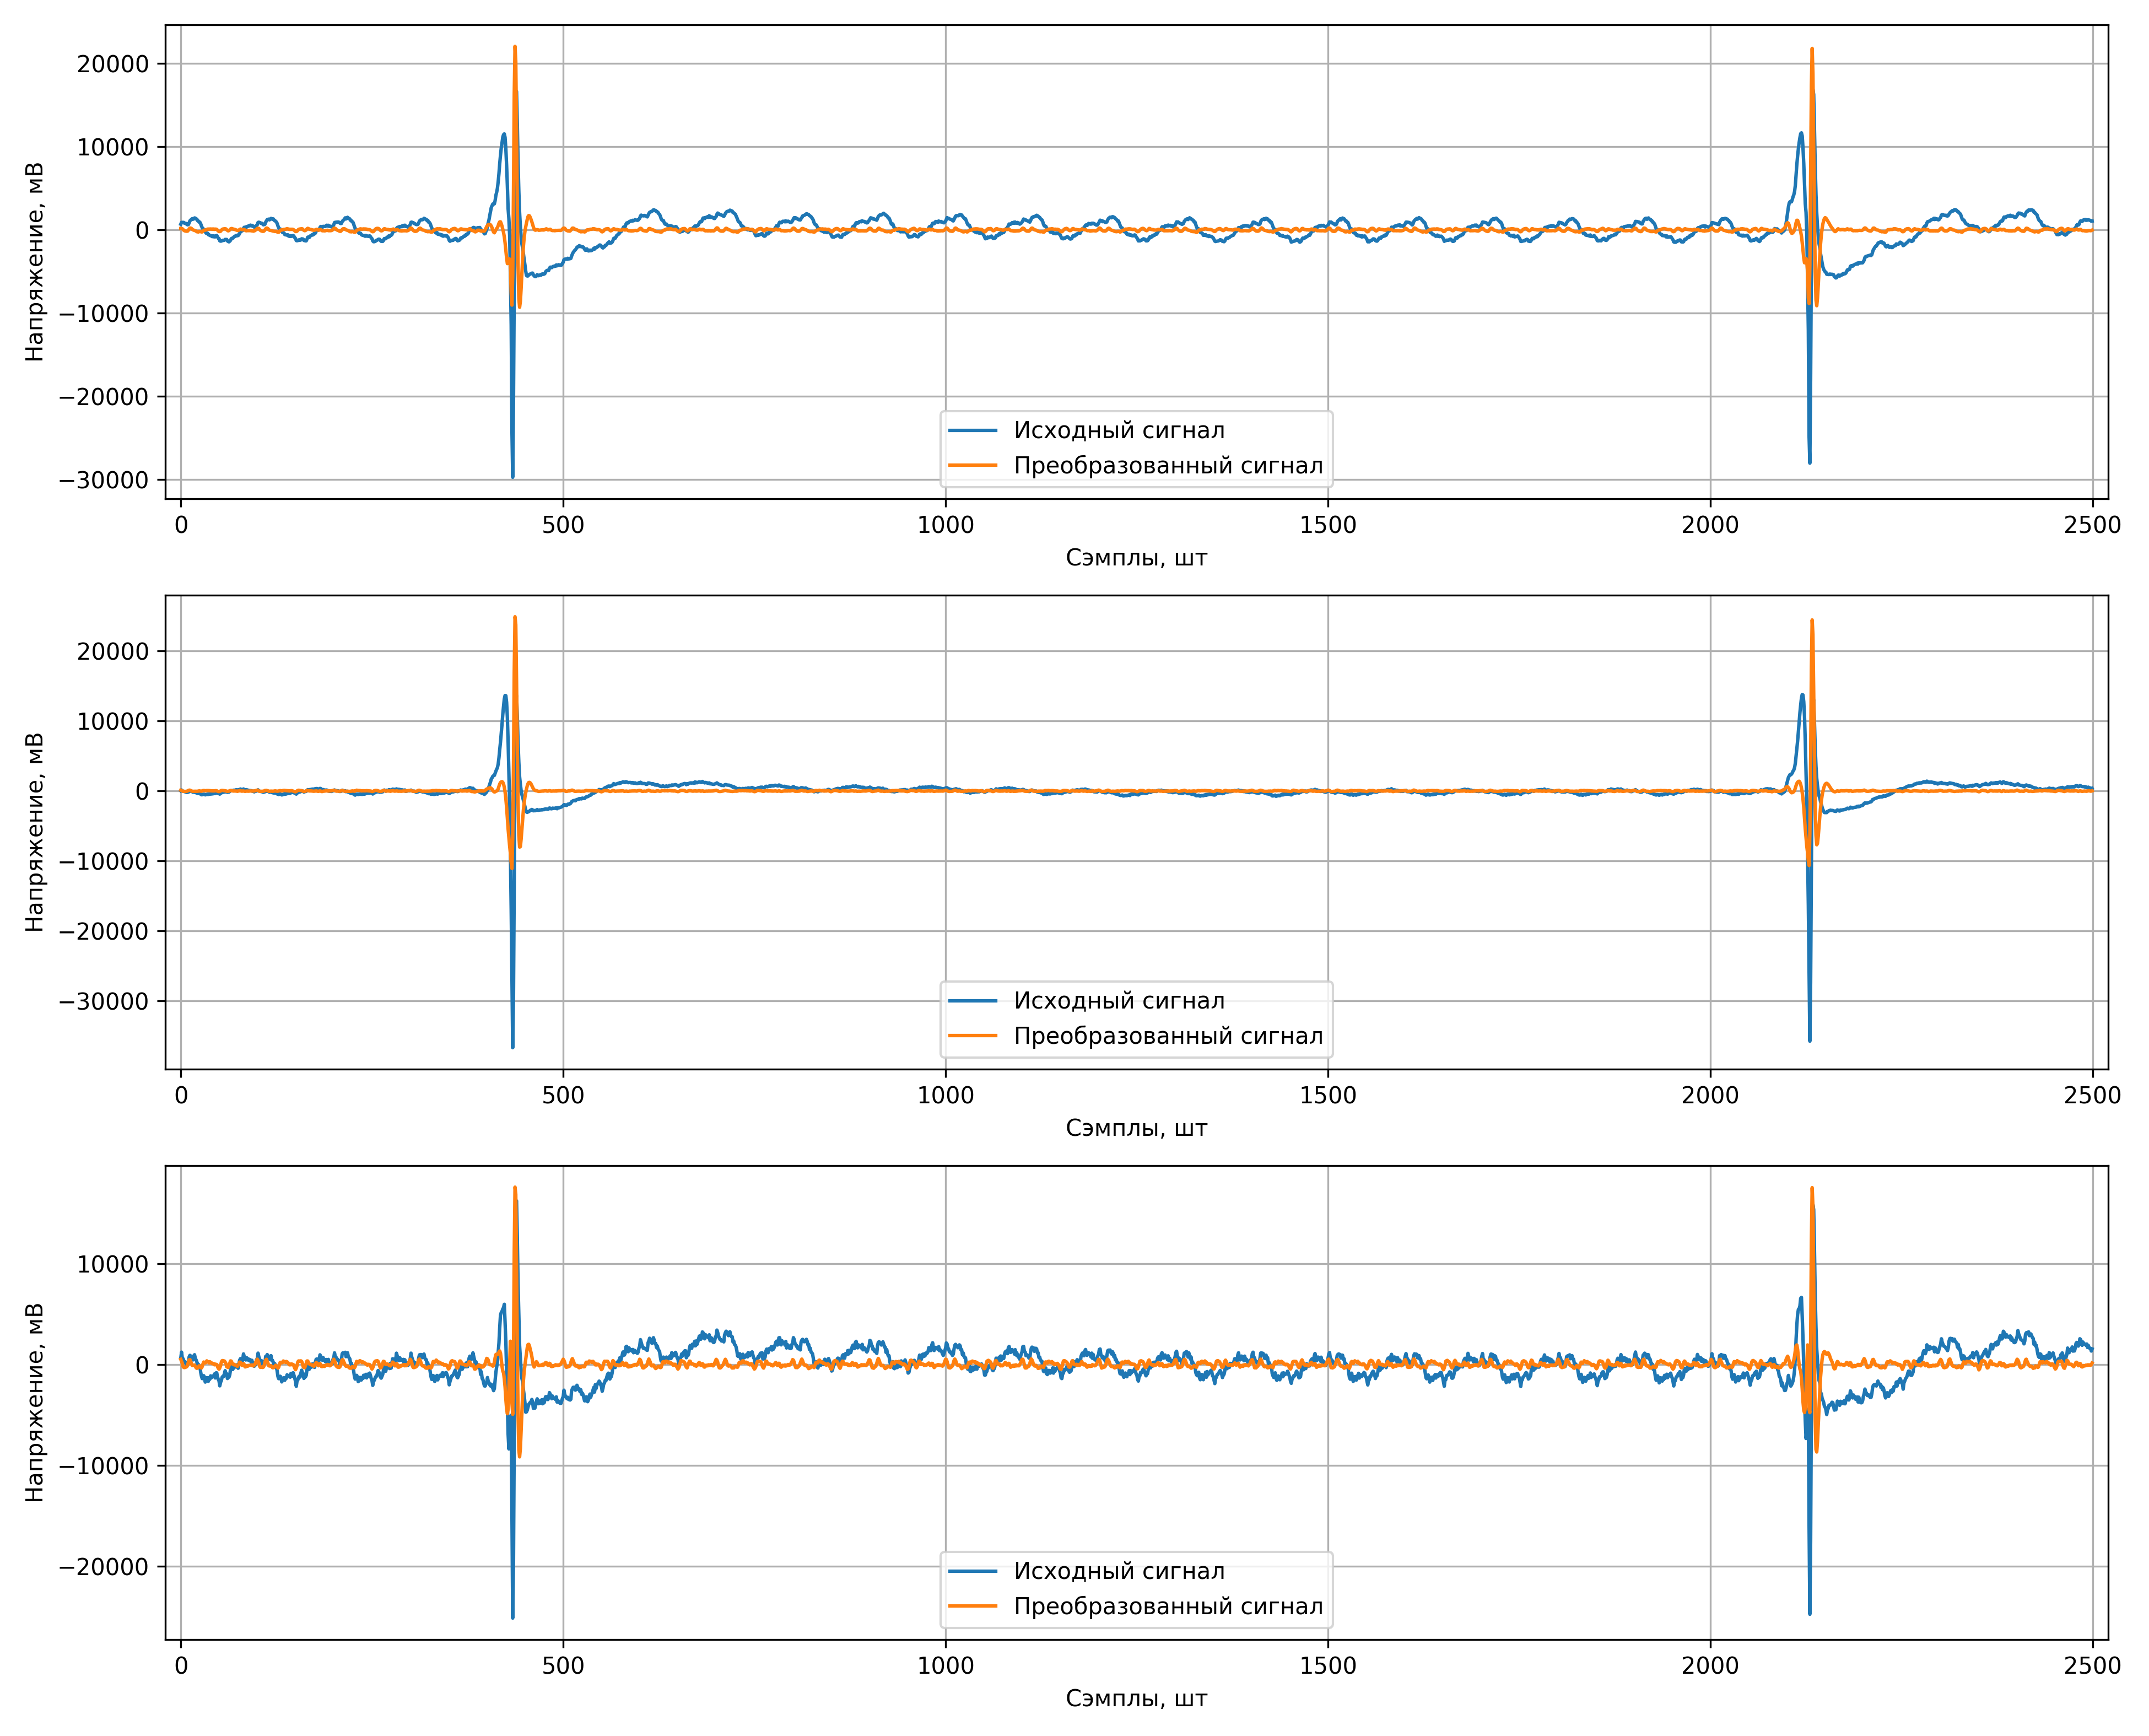
\includegraphics[width=\textwidth]{filtered}
	\caption{Преобразованный сигнал (без масштабирования)}
	\label{fig:filtered}
\end{figure}

\subsection{Предобработка разметки} Как уже было оговорено ранее, в данных
присутствует сильный дисбаланс меток активации ко всему сигналу. В связи с этим
возникает необходимость в увеличении количества меток. Достичь поставленной
цели поможет замена единичных активаций функциями унимодального типа. В
качестве такой функции использовалась плотность вероятности нормального
распределения с средним 0 и стандартным отклонением 20, отмасштабированная так,
чтобы в максимуме достигалась единица (см. рис. \ref{fig:gaussian}). Полученный
результат использовался в качестве ядра свертки для преобразования меток (см.
рис. \ref{fig:processed-label}, \ref{fig:processed-labels}).


\begin{figure}[!htb]
	\centering
	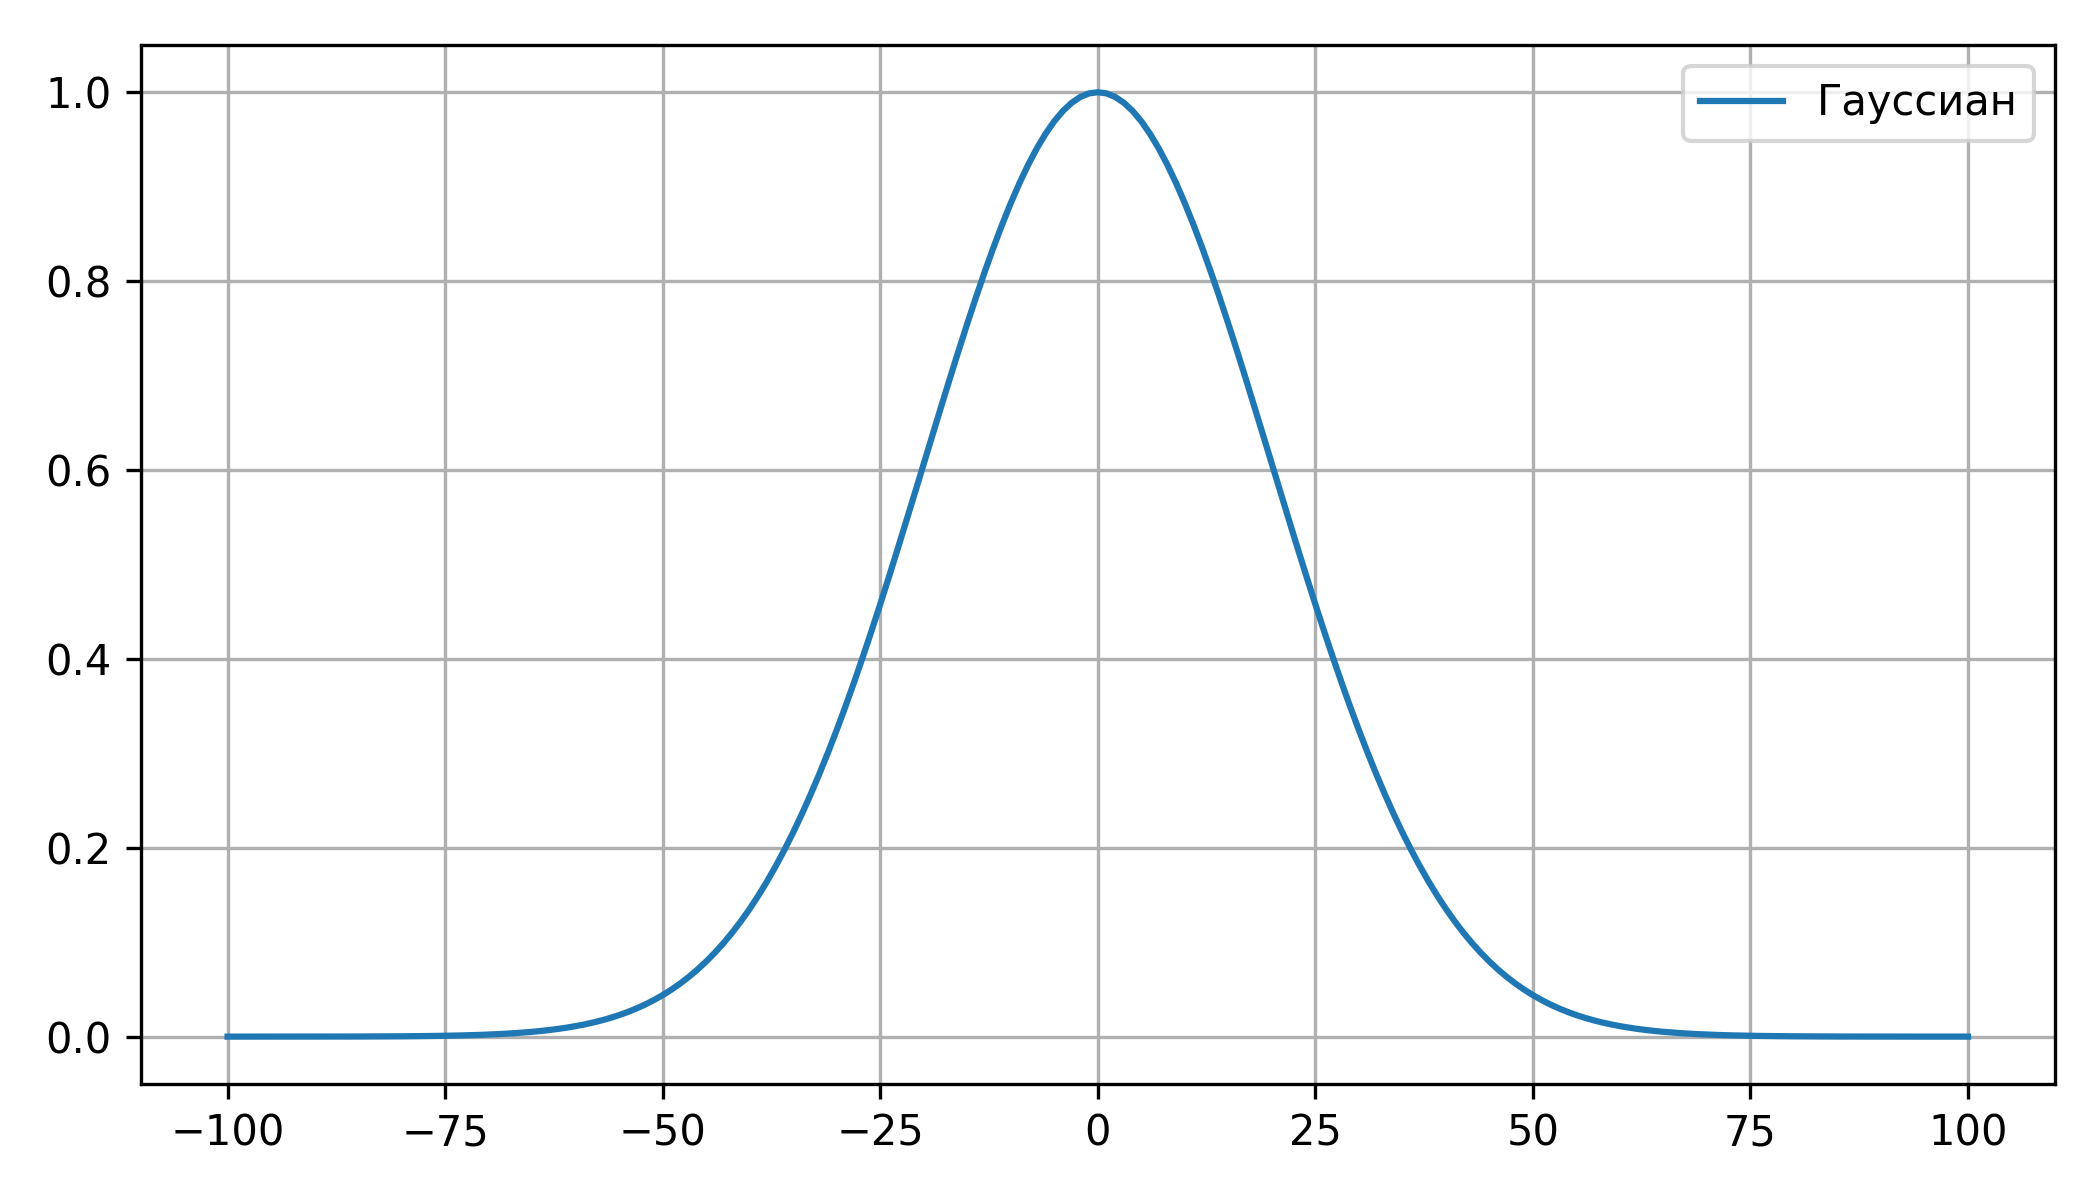
\includegraphics[width=0.7\textwidth]{gaussian}
	\caption{Ядро свертки}
	\label{fig:gaussian}
\end{figure}

\begin{figure}[!htb]
	\centering
	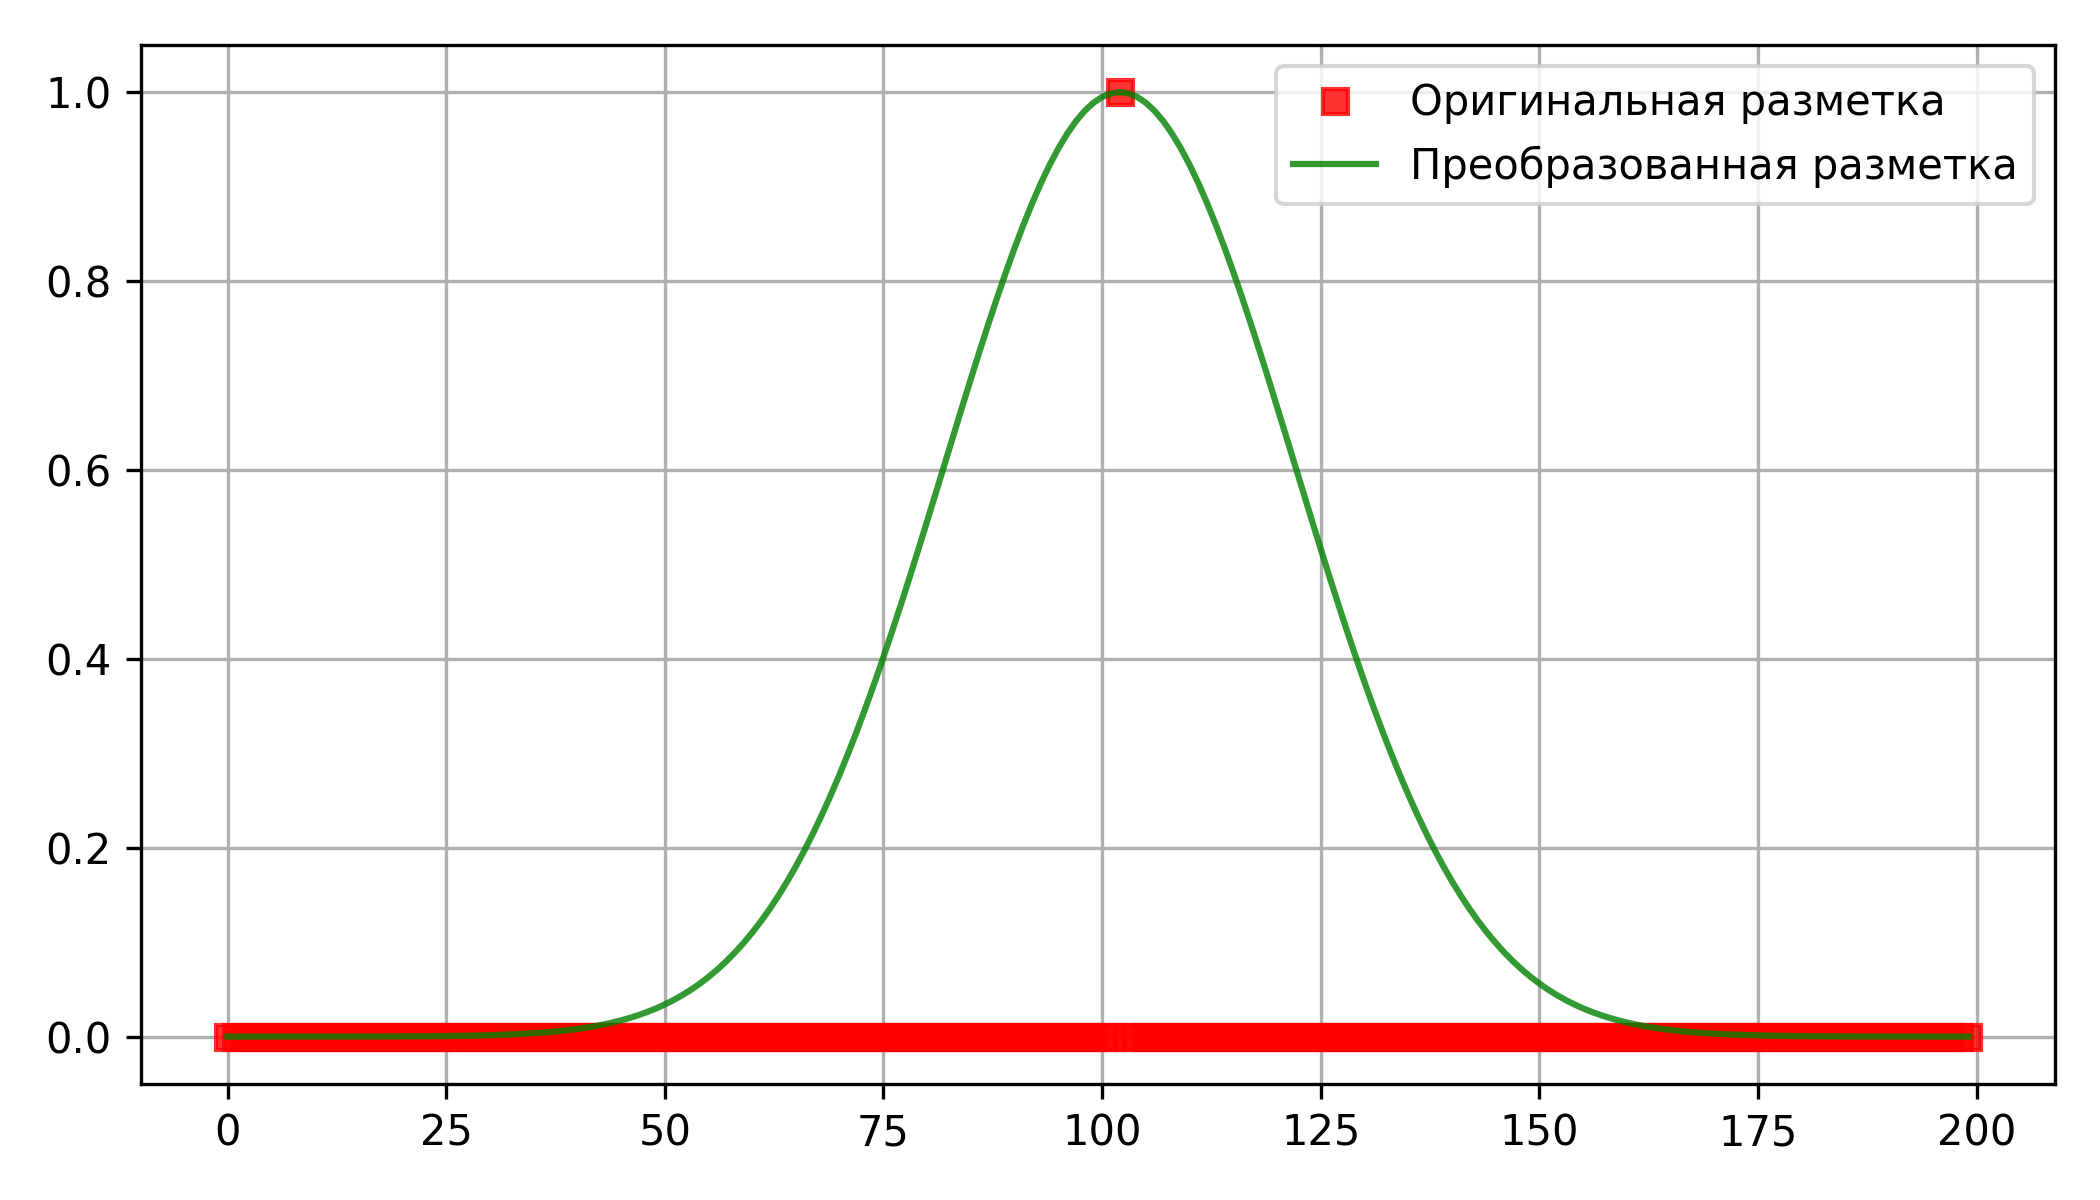
\includegraphics[width=0.7\textwidth]{processed_label}
	\caption{Преобразованная метка}
	\label{fig:processed-label}
\end{figure}

\begin{figure}[!htb]
	\centering
	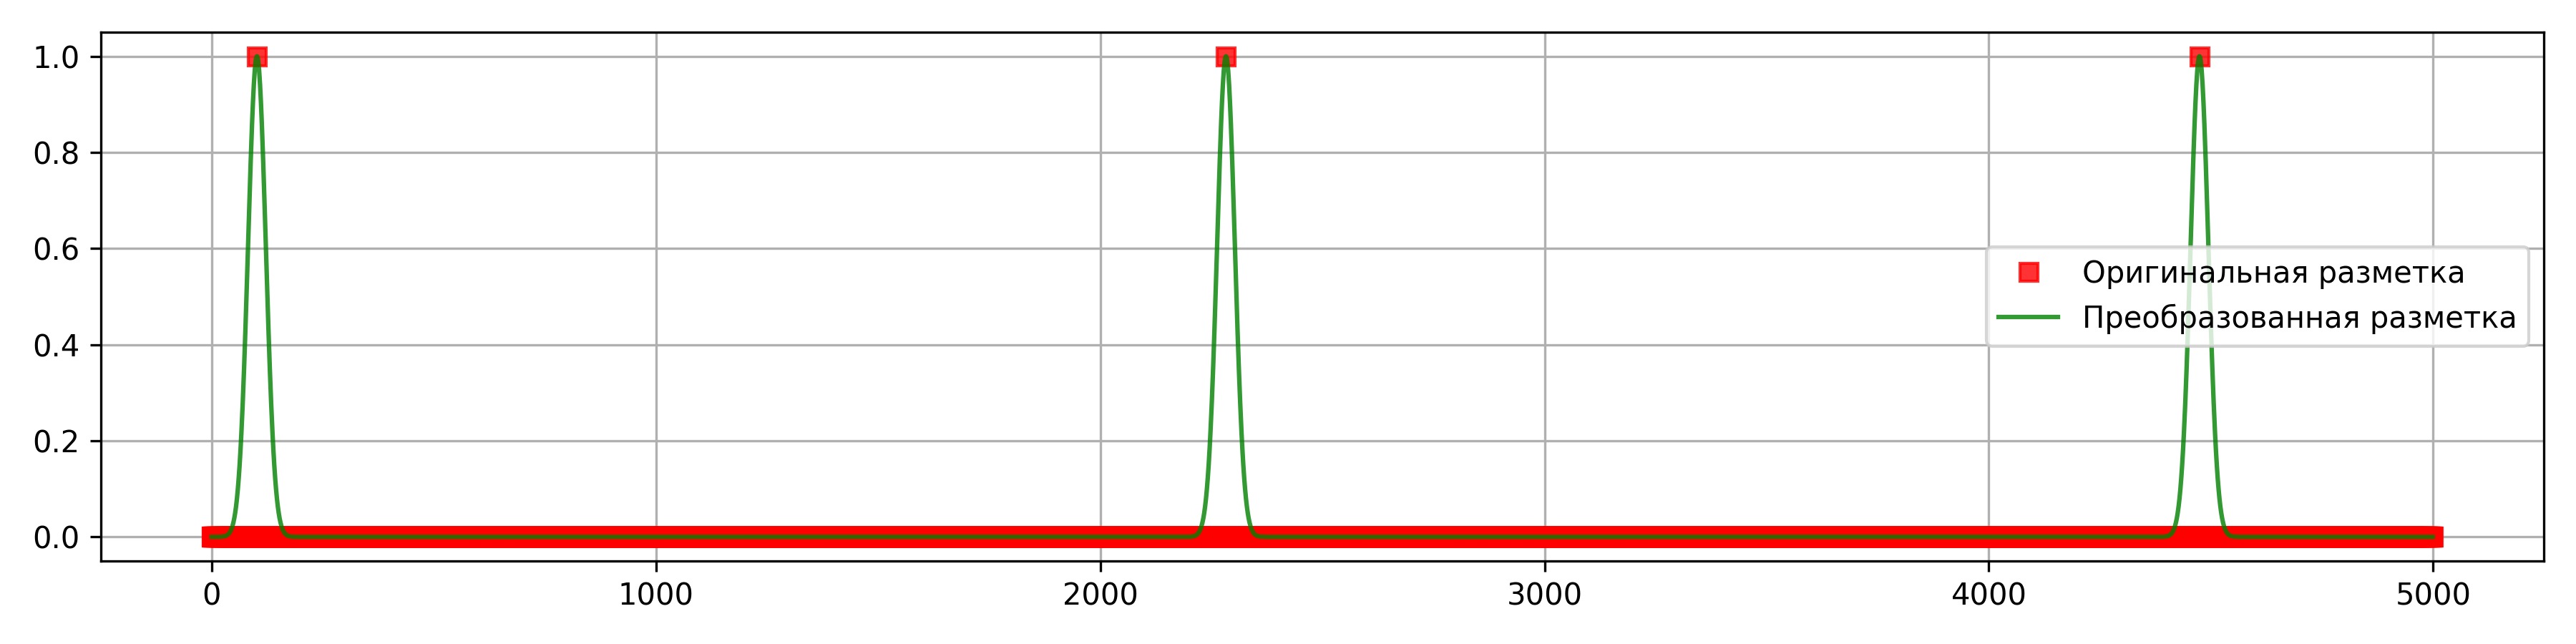
\includegraphics[width=\textwidth]{processed_labels}
	\caption{Преобразованные метки}
	\label{fig:processed-labels}
\end{figure}


\section{Результат}

В итоге получается файл dataset.csv со следующими колонками:

\begin{itemize}
	\item channel --- канал из которого взята часть сигнала
	\item experiment --- эксперимент из которого взята часть сигнала
	\item label --- относительный путь до файла разметки
	\item signal --- относительный путь до файла сигнала
\end{itemize}

\noindent, который представляет из себя набор необходимых данных для обучения
нейронных сетей и проведения экспериментов. Данный формат позволяет легко
обращаться к нужным данным в процессе обучения моделей и анализа результатов.
